\chapter{MARCO TEÓRICO}
\label{cap:marco}

% =====================================================================
\section{Metodología de Desarrollo}
\label{sec:metodologia-desarrollo}

Una metodología de desarrollo de software es un marco de trabajo que se usa
para estructurar, planificar y controlar el proceso de desarrollo de sistemas de
información (Gabriel Maide \& Pacienzia, 2020). Asimismo el objetivo de las
distintas metodologías es el intentar organizar los equipos de trabajo para que
estos desarrollen las funciones de un programa de la mejor manera posible
(Santander, 2020). Una metodología establece un conjunto de prácticas, técnicas
y procesos que permiten mejorar la eficiencia del trabajo, garantizar la
calidad y reducir la incertidumbre durante el ciclo de vida del software
(Pressman, 2010).

Las metodologías de desarrollo proporcionan lineamientos que facilitan la
coordinación del equipo, la definición clara de los requerimientos, la gestión
de riesgos y la evaluación del avance del proyecto. El uso de la metodología
adecuada contribuye a la minimización de riesgos, estandarización de
procedimientos y mejorar la productividad.

Las metodologías de desarrollo de software son enfoques que proporcionan un
marco claro para planificar, ejecutar y entregar proyectos de software, estas
pueden ser lineales o iterativas, se ajustan a diferentes tipos de proyectos y
equipos de acuerdo a las necesidades específicas de cada proyecto o equipo
(Team, 2024).

% =====================================================================
\section{Metodologías de desarrollo de software tradicionales vs ágiles}
\label{sec:tradicionales-agiles}

Las metodologías de desarrollo de software se agrupan principalmente en
tradicionales y ágiles, cada una con enfoques y características distintas.

\subsection{Metodologías tradicionales}

Las metodologías tradicionales, conocidas también como predictivas, son
enfoques secuenciales y lineales, basados en una planificación detallada y
estructurada, donde cada fase debe completarse antes de iniciar la siguiente,
tampoco se puede volver hacia atrás una vez se ha cambiado de fase. Estas
metodologías, no se adaptan nada bien a los cambios, y el mundo actual cambia
constantemente (Santander, 2020).

Este enfoque es ideal para proyectos en los que los requerimientos están bien
definidos desde el principio.

{\small
\begin{longtable}{L{2.6cm} L{6.8cm} L{5.4cm}}
\caption{Comparación de Metodologías tradicionales de desarrollo de software}
\label{tab:metodologias-tradicionales}\\
\toprule
\textbf{Metodología} & \textbf{Descripción} & \textbf{Características} \\
\midrule
\endfirsthead
\toprule
\textbf{Metodología} & \textbf{Descripción} & \textbf{Características} \\
\midrule
\endhead
\bottomrule
\endfoot
\textbf{Waterfall} & La metodología waterfall o cascada, es un proceso
secuencial, el proyecto se divide en fases, las cuales deben completarse
completamente antes de pasar a la siguiente. El avance del progreso va de
arriba hacia abajo. &
\begin{tablista}
  \item Enfoque lineal y estructurado.
  \item Requiere una planificación previa.
  \item No permite adaptaciones una vez iniciada la ejecución.
  \item Fácil de entender.
\end{tablista} \\
\midrule
\textbf{Espiral} & Esta metodología integra la gestión de riesgos a lo largo
del proceso de desarrollo. El desarrollo ocurre en ciclos o vueltas y cada uno
de estos cuenta con 4 fases: planificación, análisis de riesgos, ingeniería y
evaluación por parte del cliente. &
\begin{tablista}
  \item Enfoque iterativo basado en ciclos sucesivos.
  \item Permite incorporar ajustes o mejoras en cada iteración.
  \item Contempla análisis de riesgos periódico.
\end{tablista} \\
\midrule
\textbf{Incremental} & Esta metodología combina elementos de la metodología
cascada, permite desarrollar el producto de forma progresiva, cada etapa
incremental constituye una nueva funcionalidad, lo que permite ver resultados
de forma más rápida en comparación del modelo cascada. &
\begin{tablista}
  \item Entrega parcial del sistema.
  \item Facilita la detección de errores temprana.
  \item Recopila comentarios de clientes después de cada entrega.
  \item Flexible a los cambios.
  \item Combinación de enfoques lineales e iterativos.
\end{tablista} \\
\midrule
\textbf{Prototipado} & Esta metodología desarrolla un modelo preliminar y
tangible de software, esto permite que el usuario pruebe y de
retroalimentación, para así poder ajustar los requisitos y mejorar el diseño
del sistema final. &
\begin{tablista}
  \item Facilita la comunicación con el usuario.
  \item Reduce la incertidumbre.
  \item Es iterativa.
  \item Reduce riesgos y costos.
  \item Es flexible y versátil.
\end{tablista} \\
\midrule
\textbf{Diseño rápido de aplicaciones RAD} & Esta metodología permite
desarrollar software de alta calidad en un corto periodo de tiempo. Los costes
son mucho más altos y el desarrollo es flexible, aunque requiere mayor
intervención de los usuarios. &
\begin{tablista}
  \item Desarrollo basado en prototipos funcionales.
  \item Iteraciones cortas y desarrollo incremental.
  \item Alta participación del usuario.
\end{tablista} \\
\end{longtable}
}
\fuente{Elaboración propia.}

\conclusion{De acuerdo al análisis comparativo presentado en la
Tabla~\ref{tab:metodologias-tradicionales}, se concluye que la principal
diferencia entre las metodologías tradicionales radica en su tolerancia al
cambio y la gestión de riesgo. Mientras que el modelo cascada prioriza una
estructura secuencial y rígida, los modelos espiral, incremental y prototipado
introducen cambios iterativos que permiten la validación progresiva del
usuario. Por lo tanto, estas metodologías son más aptas para proyectos con
requerimientos claros, estables que no cambiaran con el tiempo.}

\subsection{Metodologías ágiles para móvil}

Las metodologías ágiles aplicadas al desarrollo móvil surgen como respuesta a
la necesidad de adaptarse a un entorno cambiante y a ciclos de producción
rápidos. Estas metodologías están centradas en la entrega continua de valor, la
colaboración constante con el cliente y la capacidad de adaptarse a nuevos
requerimientos.

Las metodologías ágiles son las más utilizadas en la actualidad debido a su alta
flexibilidad y agilidad (Santander, 2020). Se basan en la metodología
incremental, en la que en cada ciclo de desarrollo se agregan nuevas
funcionalidades a la aplicación final.

{\small
\begin{longtable}{L{2.4cm} L{7.2cm} L{5.2cm}}
\caption{Comparación de metodologías ágiles móviles}
\label{tab:metodologias-agiles}\\
\toprule
\textbf{Metodología} & \textbf{Descripción} & \textbf{Características} \\
\midrule
\endfirsthead
\toprule
\textbf{Metodología} & \textbf{Descripción} & \textbf{Características} \\
\midrule
\endhead
\bottomrule
\endfoot
\textbf{Scrum} & Es una metodología ágil, que divide los requerimientos y
tareas de forma similar a Kanban. Está compuesto por iteraciones fijas y cortas
denominadas Sprints, así como una estructura basada en roles, eventos y
artefactos definidos. Su objetivo es entregar incrementos funcionales del
producto en ciclos de 2 a 4 semanas, fomentando la colaboración y la
inspección continua (Schwaber \& Sutherland, 2020). &
\begin{tablista}
  \item Roles definidos (Product Owner, Scrum Master, Equipo).
  \item Iteraciones cortas y fijas.
  \item Entregas incrementales al final de cada sprint.
  \item Alta colaboración con el cliente.
  \item Uso de backlog y tableros para la gestión visual del trabajo.
  \item[] (Schwaber \& Sutherland, 2020)
\end{tablista} \\
\midrule
\textbf{Extreme Programming (XP)} & Es una metodología basada en relaciones
interpersonales, la colaboración y la retroalimentación continua. Su objetivo
principal es crear un entorno de trabajo basado en la comunicación constante,
simplicidad del diseño y participación activa del cliente. Incorpora prácticas
de ingeniería como pair programming, test-driven development, refactorización
constante e integración continua (Beck \& Andres, 2005). &
\begin{tablista}
  \item Trabajo colaborativo.
  \item Diseño sencillo y adaptables.
  \item Desarrollo guiado por pruebas.
  \item Refactorización continua.
  \item Integración continua.
  \item Entregas frecuentes y pequeñas iteraciones.
  \item Planificación basada en historias de usuario.
  \item Programación en parejas.
\end{tablista} \\
\midrule
\textbf{Mobile-D} & Es una metodología ágil para el desarrollo de aplicaciones
móviles para equipos pequeños, está centrada en ciclos de desarrollo rápidos y
entrega continua. Combina prácticas ágiles con procesos orientados al hardware
y ciclos muy cortos de entrega (Abrahamsson, y otros, 2004). &
\begin{tablista}
  \item Diseñada para desarrollo móvil.
  \item Iteraciones rápidas.
  \item Adaptación a restricciones de hardware.
  \item Enfocado en grupos pequeños.
\end{tablista} \\
\midrule
\textbf{Kanban} & Es una metodología de trabajo inventada por la empresa de
automóviles Toyota. Consiste en dividir las tareas en porciones mínimas y
organizarlas en un tablero de trabajo dividido en tareas pendientes, en curso y
finalizadas. De esta forma se crea un flujo de trabajo muy visual basado en
tareas prioritarias e incrementando el valor del producto (Santander, 2020). &
\begin{tablista}
  \item Visualización del trabajo.
  \item Límite de trabajo en curso.
  \item Mejora continua.
  \item No requiere iteraciones fijas.
  \item Fácil implementación en equipos individuales.
  \item Gestión visual del trabajo.
\end{tablista} \\
\end{longtable}
}
\fuente{Elaboración propia a partir de (Schwaber \& Sutherland, 2020); (Beck \&
Andres, 2005); (Santander, 2020); (Abrahamsson, y otros, 2004).}

\conclusion{En conclusión, todas las metodologías ágiles comparten principios
como la flexibilidad y la entrega continua, sin embargo, la metodología
Mobile-D es la más adecuada para proyectos móviles por su rapidez, sus
iteraciones cortas y su adaptación a las particularidades del hardware.}

% =====================================================================
\section{Mobile-D}
\label{sec:mobile-d}

La metodología Mobile-D es un enfoque ágil diseñado para el desarrollo de
software en dispositivos móviles. Surgió como resultado de investigaciones
realizadas por el VTT, con el objetivo de responder a los desafíos propios del
entorno móvil, como ciclos de producción acelerados, restricciones de hardware,
diversidad de plataformas y cambios frecuentes en los requisitos (Abrahamsson
et al., 2004).

Mobile-D es adecuada para proyectos que requieren rapidez, flexibilidad y alta
calidad, como aplicaciones de seguridad informática, plataformas de comercio
electrónico, aplicaciones de simulación entre otros. Está pensada para equipos
pequeños. Esta metodología combina prácticas de diversas metodologías ágiles,
como Scrum, XP y prácticas de ingeniería de software.

\subsection{Fases y etapas}

El desarrollo mediante el enfoque de Mobile-D se compone de 5 fases como se
muestra en la Figura~\ref{fig:mobile-d}, estas fases son: Exploración,
Inicialización, Producción, Estabilización y Pruebas del sistema.

\begin{figure}[H]
    \centering
    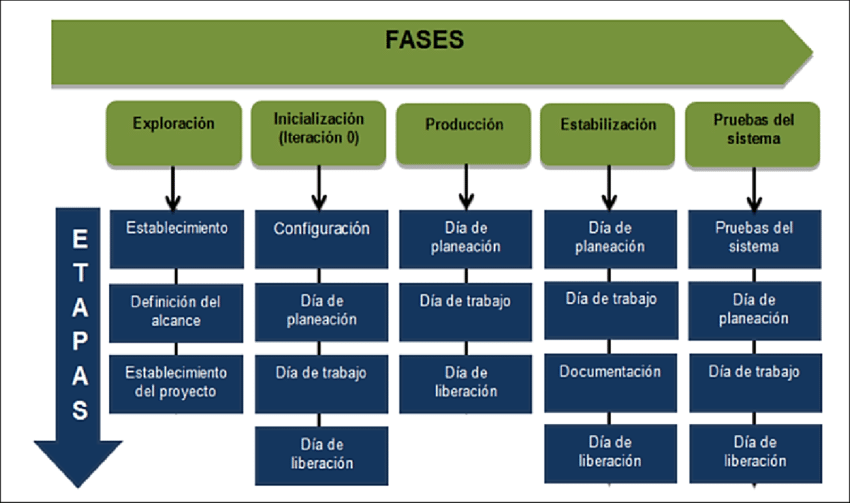
\includegraphics[width=0.85\textwidth]{figuras/docx/mobile-d-fases.png}
    \caption{Fases y etapas de la metodología Mobile-D (Leyva, León, \& García, 2016)}
    \label{fig:mobile-d}
\end{figure}

\begin{itemize}
    \item \textbf{Fase de Exploración}

    Esta es la fase inicial donde se define el proyecto y se establecen las
    bases técnicas y organizativas. En esta fase se definen los objetivos, el
    alcance, los actores involucrados y las restricciones técnicas y
    funcionales del proyecto. También se seleccionan las tecnologías
    principales y se configura el entorno de trabajo.

    \item \textbf{Fase de Inicialización}

    En esta fase se prepara el equipo, las herramientas y la arquitectura
    técnica para comenzar las iteraciones de desarrollo. Dentro de esta fase se
    verifican los recursos humanos, tecnológicos y físicos que se necesitarán.
    Esta fase se divide en cuatro etapas: la puesta en marcha del proyecto, la
    planificación inicial, el día de prueba y día de salida (Gómez \&
    Hernández, 2016).

    \item \textbf{Fase de Producción}

    Esta fase se caracteriza por el uso de ciclos cortos e incrementales. En
    esta etapa se implementan funcionalidades mediante prácticas de desarrollo
    guiado en pruebas TDD, la integración continua y el desarrollo iterativo.
    Su objetivo principal es construir versiones funcionales del producto de
    manera progresiva, garantizando la calidad y retroalimentación constante
    durante todo el proceso.

    \item \textbf{Fase de Estabilización}

    En esta fase se integran los componentes generados durante la producción
    para asegurar que el sistema funcione correctamente. Esta etapa los
    desarrolladores optimizan el rendimiento, mejoran la consistencia interna
    del software y realizan las refactorizaciones necesarias. No se añaden
    nuevas funcionalidades, sino que se fortalece la calidad general del
    producto.

    \item \textbf{Fase de Pruebas}

    En esta fase se verifica que la aplicación cumpla con los requerimientos
    funcionales y de calidad definidos al inicio del proyecto. Esta etapa
    incluye pruebas de aceptación, pruebas de dispositivos reales y corrección
    de errores detectados. El propósito de esta etapa es garantizar que el
    sistema sea estable, usable y se encuentre listo para ser entregado al
    cliente o desplegado en un entorno final.
\end{itemize}

% =====================================================================
\section{Programación Móvil}
\label{sec:programacion-movil}

La programación móvil consiste en diseñar, implementar, probar y desplegar
software que se ejecuta en dispositivos móviles. Este tipo de desarrollo de
software tiene como objetivo crear aplicaciones que se ejecuten en varios
dispositivos móviles, incluidos Android, iOS y otras plataformas menos
populares. La plataforma móvil abarca dos enfoques principales de desarrollo
nativo y multiplataforma (AppMaster, 2023).

Una aplicación móvil se define como un software diseñado para ejecutarse en
dispositivos portátiles como teléfonos inteligentes y tabletas, con el fin de
realizar tareas específicas para el usuario (Apps, 2011).

En el ámbito de desarrollo de software, los sistemas operativos móviles
dominantes son Android y iOS, los cuales concentran prácticamente la totalidad
del mercado global de smartphones. Android, mantenido por Google, es un sistema
abierto basado en Linux que ofrece gran flexibilidad, soporte para múltiples
fabricantes y acceso a herramientas de desarrollo como Android Studio y las
bibliotecas Jetpack (Google, 2023). Por su parte, iOS desarrollado por Apple, se
caracteriza por ser un sistema operativo cerrado, de alto control de calidad,
diseñado exclusivamente para ejecutarse en el hardware de Apple y herramientas
como Xcode y SwiftUI que permiten crear aplicaciones con elevado rendimiento y
experiencia de usuario (Apple, 2023).

{\small
\begin{longtable}{L{3.6cm} L{5.9cm} L{5.3cm}}
\caption{Comparación de Android vs iOS}
\label{tab:android-ios}\\
\toprule
\textbf{Características} & \textbf{Android} & \textbf{iOS} \\
\midrule
\endfirsthead
\toprule
\textbf{Características} & \textbf{Android} & \textbf{iOS} \\
\midrule
\endhead
\bottomrule
\endfoot
\textbf{Propietario} & Google & Apple \\
\textbf{Familia S.O.} & Linux & UNIX \\
\textbf{Tipo de licencia} & Código abierto & Código cerrado y propietario \\
\textbf{Programado en} & C, C++, Java & Swift, Objective-C, C, C++ \\
\textbf{Lenguajes de programación} & Java, Kotlin & Swift \\
\textbf{Entorno de desarrollo} & Android Studio & Xcode \\
\textbf{Arquitectura del sistema} & Basada en kernel Linux + HAL + Runtime ART
& Basada en kernel XNU + frameworks de alto nivel \\
\textbf{Presencia en el mercado boliviano} & 90.74\,\% (Global, 2025) &
8.7\,\% (Global, 2025) \\
\textbf{Diseño} & Diseños flexibles, personalizado, colorido, adaptable a
muchas marcas y dispositivos. & Diseño minimalista, elegante, limpio y
extremadamente consistente. \\
\textbf{Personalización} & Permite la personalización de la interfaz mediante
launchers personalizados, permite utilizar paquetes de temas, ajustar el panel
de configuración rápida y modificar el comportamiento de aplicaciones
predeterminadas (Gironés, 2012). & Su personalización es limitada, prioriza la
simplicidad, estabilidad y coherencia visual, lo que reduce riesgos de
incompatibilidad (Apple, 2023). \\
\textbf{Fragmentación} & Samsung, Huawei, Xiaomi, Motorola, Sony. & Exclusivo
para dispositivos Apple (iPhone, iPad). \\
\textbf{Distribución de Apps} & Play Store y permite instalación manual
(APK/Sideloading). & App Store \\
\textbf{Asistente Virtual} & Google Now, Google Assistant & Siri \\
\end{longtable}
}
\fuente{Elaboración propia.}

\conclusion{En conclusión, Android destaca por su capacidad de adaptabilidad, y
su compatibilidad con distintos lenguajes de programación, lo que lo hace más
versátil; su flexibilidad y escalabilidad lo hacen la plataforma idónea para el
desarrollo de una aplicación móvil.}

% =====================================================================
\section{Sistema Operativo}
\label{sec:sistema-operativo}

\subsection{Android}

Android es un sistema operativo y una plataforma de desarrollo libre basada en
Linux y de código abierto desarrollado por Google (Tomás, 2019). Este sistema
operativo es utilizado en tablets, netbooks, reproductores de música e incluso,
PC's (Sanz, 2019). Hoy en día podemos encontrar relojes, gafas, cámaras, TV,
sistema para automóviles, electrodomésticos y una gran variedad de sistemas
empotrados que se basan en este sistema operativo por lo que lo hace adaptable
a cualquier tipo de hardware (Tomás, 2019).

Su dominio en el mercado global, superando el 70\,\% de cuota del mercado, y su
prevalencia superior al 90\,\% en el contexto boliviano, lo posicionan como el
estándar en el desarrollo Mobile en la región (Global, 2025). El desarrollo
Android ha ido evolucionando puesto que permite que fabricantes,
desarrolladores y la comunidad global adapten el sistema, añadiendo funciones
nuevas y personalicen la interfaz, lo que facilita la creación de aplicaciones
innovadoras y la configuración del sistema a distintos entornos y necesidades
(Alliance, 2022).

\subsection{Arquitectura de Android}

Desde una perspectiva técnica, Android se compone de cuatro capas principales.
En la base se encuentra el kernel de Linux, responsable de gestionar procesos,
la administración de memoria y la seguridad del sistema. Sobre él se ubica la
capa del Hardware Abstraction Layer (HAL), que permite que diferentes
fabricantes integren su propio hardware. La tercera capa de las APIs de
Android, que ofrecen servicios como gráficos, multimedia, ubicación y
sensores. Finalmente, el framework de aplicaciones, que facilita la creación de
aplicaciones mediante bibliotecas de alto nivel y componentes como Activities,
Services y Content Providers (Meier \& Lake, 2018).

El siguiente gráfico muestra la arquitectura de Android. Como se puede observar
en la Figura~\ref{fig:arquitectura-android}, su arquitectura se encuentra
formada por cuatro capas.

\begin{figure}[H]
    \centering
    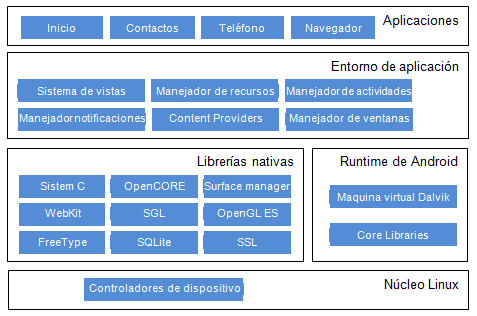
\includegraphics[width=0.75\textwidth]{figuras/docx/arquitectura-android.png}
    \caption{Arquitectura de Android (Gómez A. A., 2015)}
    \label{fig:arquitectura-android}
\end{figure}

\subsection{Ventajas y limitaciones}

Android destaca por que ofrece ventajas como:

\begin{itemize}
    \item Flexibilidad para funcionar en múltiples tipos de hardware.
    \item Libertad de personalización de interfaz.
    \item Libertad de configuración del sistema.
    \item Compatibilidad amplia con una gran variedad de herramientas y
    servicios de Google.
    \item Alta calidad de gráficos y sonido.
    \item Portabilidad garantizada, ya que sus aplicaciones son desarrolladas en
    Java.
    \item Nivel de seguridad aceptable.
\end{itemize}

Sin embargo, esto también genera limitaciones, como la fragmentación entre
dispositivos y diferentes velocidades en la distribución de actualizaciones del
sistema.

% =====================================================================
\section{Realidad Aumentada}
\label{sec:realidad-aumentada}

La realidad aumentada (RA) es una combinación visual de elementos reales y
virtuales que interaccionan entre ellos (Navarro, Martínez, \& Martínez, 2018),
también es la integración en tiempo real de la información digital en el
entorno de un usuario. La tecnología de RA superpone el contenido al mundo
real, lo que enriquece la percepción de la realidad del usuario en lugar de
reemplazarla (Hayes \& Downie, 2025). A diferencia de la realidad virtual, que
sustituye completamente el entorno físico, la RA superpone información digital
como imágenes, modelos 3D, texto o animaciones sobre la realidad observada a
través de dispositivos como smartphones, tablets o lentes inteligentes (Azuma,
1997).

\subsection{Componentes de un sistema de Realidad Aumentada}

Un sistema de Realidad Aumentada es una convergencia de hardware y software que
opera un bucle continuo de retroalimentación, en otras palabras, un sistema de
RA debe cumplir con tres características principales, combinar lo real y lo
virtual, operar interactivamente y registrar elementos en 3D (Azuma, 1997).

Un sistema de RA incluye los siguientes componentes esenciales:

\begin{itemize}
    \item \textbf{Dispositivo de visualización:} Permite mostrar la mezcla entre
    la imagen real y los elementos virtuales. Puede ser un teléfono móvil,
    tablet, gafas inteligentes o pantalla montada en la cabeza (Head-Mounted
    Display).
    \item \textbf{Cámara o sensores de captura:} Registra el entorno físico para
    detectar superficies, marcadores o puntos de referencia. Por ejemplo:
    cámaras RGB, sensores de profundidad, giroscopio, acelerómetro.
    \item \textbf{Módulo de seguimiento (tracking):} Se encarga de identificar la
    posición y orientación del usuario o del dispositivo. Esto incluye:
    marker-based, markerless, SLAM, reconocimiento de superficies.
    \item \textbf{Motor de renderizado:} Genera y superpone objetos virtuales en
    el entorno real con coherencia visual y espacial.
    \item \textbf{Interfaz de interacción:} Permite al usuario manipular objetos
    virtuales mediante gestos, toques o movimiento.
\end{itemize}

\subsection{Tecnologías para el desarrollo de Realidad aumentada móvil}

Para el desarrollo móvil, las principales tecnologías de RA son:

\begin{itemize}
    \item \textbf{ARCore:} Es el SDK de realidad aumentada de Google que ofrece
    APIs multiplataforma para crear nuevas experiencias envolventes en Android,
    iOS, Unity y la Web. Transforma la manera en que las personas juegan,
    compran, aprenden, crean y experimentan el mundo juntas mediante la
    comprensión contextual de las personas, los lugares y las cosas
    (Developers, 2025).
    \item \textbf{ARKit:} Es un framework de Apple, altamente optimizado y
    compatible con sensores avanzados como LiDAR. Permite capturar
    impresionantes videos de alta resolución perfectos para la edición de video
    profesional, producción cinematográfica, aplicaciones de redes sociales
    entre otros (Inc., 2025).
\end{itemize}

% =====================================================================
\section{Inteligencia Artificial}
\label{sec:inteligencia-artificial}

La inteligencia artificial (IA) es una tecnología transformadora que permite a
las máquinas llevar a cabo tareas de resolución de problemas similares a las de
los humanos. Desde el reconocimiento de imágenes y la generación de contenido
creativo hasta la creación de predicciones basadas en datos, la IA permite a
las empresas tomar decisiones más inteligentes a escala (Services, 2025).

La IA consiste en enseñar a las computadoras a hacer las actividades increíbles
que nuestros cerebros pueden hacer, desde comprender el mundo que las rodea
hasta aprender temas nuevos y generar ideas originales (Cloud, 2025). En el
contexto de las aplicaciones móviles, la IA permite integrar funciones
avanzadas como la personalización del contenido, la detección automática de
movimiento, el análisis de rendimiento del usuario y la interacción mediante
voz a texto.

\subsection{Aprendizaje automático}

El aprendizaje automático o Machine Learning es una subárea de la inteligencia
artificial dedicado a comprender y construir métodos para imitar la forma en
que aprenden los humanos (Pykes, 2024). El aprendizaje automático, es la
capacidad que tiene un programa para mejorar su desempeño en una tarea a partir
de la experiencia acumulada (Mitchell, 1997).

\subsection{Redes neuronales}

Una red neuronal es un programa o modelo de machine learning que toma
decisiones de forma similar al cerebro humano, al emplear procesos que imitan
la forma en que las neuronas biológicas trabajan juntas para identificar
fenómenos, sopesar opciones y llegar a conclusiones. Se basan en datos de
entrenamiento para aprender y mejorar su precisión con el tiempo (IBM, 2025).

\subsection{Visión por computadora}

La visión artificial es un campo de la inteligencia artificial, que permite a
los ordenadores y sistemas interpretar y analizar datos visuales, así como
también obtener información pertinente a partir de imágenes digitales, videos
y otros datos visuales (Cloud, 2025). En el contexto de las aplicaciones
móviles modernas, permite interpretar información visual mediante algoritmos
que detectan objetos, poses, personas entre otras características del entorno.

\subsection{Modelos de lenguaje Extenso (LLM)}

Los modelos de lenguaje, son modelos básicos entrenados sobre inmensas
cantidades de datos, lo que los hace capaces de comprender y generar lenguaje
natural y otros tipos de contenido para realizar una amplia variedad de
tareas. Por lo general, los LLM se basan en arquitecturas de aprendizaje
profundo, como Transformer, desarrollado por Google en 2017, y se pueden
entrenar con miles de millones de textos y otros tipos de contenido.

Debido a su escalabilidad, los LLM se pueden entrenar con otros tipos de datos,
como código, imágenes, audio y video, entre otros (Cloud, 2025). Su
versatilidad y capacidad de aprendizaje los convierten en herramientas clave en
el desarrollo de aplicaciones modernas, incluyendo sistemas móviles
inteligentes y soluciones que integren realidad aumentada e inteligencia
artificial.

% =====================================================================
\section{Fundamentos del entrenamiento físico}
\label{sec:entrenamiento}

\subsection{Entrenamiento físico}

El entrenamiento es un conjunto de ejercicios y actividades que se realizan
regularmente para mejorar la salud y el estado físico de una persona. Este tipo
de entrenamiento puede incluir variedad de actividades, cada una enfocada en
diferentes aspectos del cuerpo y objetivos personales (Orientanet, s.f.).

Hoy en día, la tecnología como sensores, aplicaciones móviles, realidad
aumentada e inteligencia artificial permiten un monitoreo exhaustivo de la
técnica y el análisis del movimiento, ofreciendo retroalimentación
personalizada en tiempo real. Estas innovaciones no solo optimizan el
rendimiento de los usuarios, sino que también garantizan que quienes están
comenzando su camino en el ejercicio puedan realizar las actividades de manera
segura y eficaz, contribuyendo de esta manera a la reducción de riesgo de
lesiones y fomentando un estilo de vida saludable.

\subsection{Principios del entrenamiento físico}

El entrenamiento físico está fundamentado en tres principios esenciales, estos
son:

\begin{itemize}
    \item \textbf{Fuerza:} Se centra en incrementar la capacidad del músculo para
    generar tensión, mediante ejercicios con resistencias progresivas. Esto no
    solo mejora el rendimiento deportivo, sino que también contribuye a la salud
    articular y la densidad ósea.
    \item \textbf{Técnica:} Implica la ejecución correcta de cada movimiento para
    maximizar los beneficios y minimizar riesgos. Una técnica adecuada asegura
    que el estímulo recae sobre los músculos deseados y evita compensaciones
    que puedan generar lesiones.
    \item \textbf{Hipertrofia:} Busca aumentar el tamaño del músculo mediante
    cargas, repeticiones y volúmenes adecuados. La hipertrofia requiere un
    equilibrio entre sobrecarga progresiva, nutrición y recuperación para
    generar crecimiento muscular efectivo.
\end{itemize}

\subsection{Biomecánica básica}

La biomecánica estudia el movimiento del cuerpo humano aplicando principios
mecánicos. Comprenderla permite optimizar los ejercicios, analizar palancas,
ángulos de articulaciones y fuerza aplicada, lo que mejora la eficiencia y
reduce el riesgo de lesiones. Los aspectos clave incluyen la alineación
corporal, el centro de gravedad, estabilidad y amplitud de movimiento.

La biomecánica proporciona las bases para corregir patrones de movimiento
disfuncionales, los cuales pueden surgir por hábitos sedentarios,
desequilibrios musculares o mala ejecución repetida de ejercicios. Identificar
estos patrones permite intervenir de manera temprana mediante correcciones
técnicas, fortalecimiento de músculos estabilizadores o ajustes en la postura.

\subsection{Lesiones comunes por mala técnica}

La técnica incorrecta en la ejecución de ejercicios, es una de las principales
causas de las lesiones en entornos de entrenamiento físico, especialmente en
principiantes. La evidencia científica demuestra que una postura inadecuada, la
falta de control motor y el uso de cargas excesivas incrementan el riesgo de
daño musculoarticular (Kolt \& Snyder-Mackler, 2007).

El desconocimiento de la técnica o la negligencia en la postura pueden provocar
lesiones frecuentes, como:

\begin{itemize}
    \item Dolor lumbar por levantamiento incorrecto de peso.
    \item Tendinitis por movimientos repetitivos sin control.
    \item Esguinces o distensiones musculares por falta de calentamiento o
    postura incorrecta.
    \item Lesiones articulares en hombros, rodillas o muñecas por sobrecarga o
    ángulos inadecuados.
\end{itemize}

Prevenir estas lesiones requiere educación, supervisión y el uso de tecnologías
de monitoreo como sensores de movimiento y análisis de video.

\subsection{Máquinas de gimnasio}

Una máquina de gimnasio es un equipo diseñado para facilitar la realización de
ejercicios físicos de manera controlada, segura y específica. Estas máquinas
están construidas con estructuras metálicas, poleas, cables, placas de peso o
mecanismos electrónicos que permiten guiar el movimiento del usuario. Su diseño
busca aislar determinados grupos musculares, mejorar la estabilidad durante el
ejercicio y proporcionar una carga regulable para adaptarse al nivel de cada
persona.

Las máquinas de gimnasio sirven para entrenar diferentes capacidades físicas
como fuerza, resistencia muscular, estabilidad y acondicionamiento
cardiovascular. Proporcionan un entorno controlado donde el usuario puede
ejecutar movimientos guiados que reducen el riesgo de lesiones, especialmente
en personas principiantes o en rehabilitación. También permiten trabajar grupos
musculares específicos con mayor precisión, mejorar la postura durante el
ejercicio y mantener una progresión segura mediante cargas ajustables. Además,
algunas máquinas monitorean parámetros como ritmo cardíaco, velocidad o
calorías, facilitando el seguimiento del rendimiento.

Las máquinas de gimnasio pueden clasificarse de diversas formas, pero las
categorías más comunes son:

\begin{itemize}
    \item \textbf{Según su función principal}
    \begin{itemize}
        \item \textit{Máquinas de fuerza o resistencia:} utilizan poleas,
        cables, placas de peso o sistemas hidráulicos para trabajar grupos
        musculares específicos. Ejemplos: prensa de piernas, máquina de pecho,
        jalón al pecho, curl de bíceps.
        \item \textit{Máquinas cardiovasculares:} diseñadas para mejorar la
        resistencia cardiorrespiratoria y quemar calorías. Ejemplos:
        caminadoras, bicicletas estáticas, elípticas, remadoras.
    \end{itemize}
    \item \textbf{Según el tipo de movimiento}
    \begin{itemize}
        \item \textit{Movimiento guiado:} la máquina controla la trayectoria
        del movimiento. Son ideales para principiantes.
        \item \textit{Movimiento libre asistido:} permiten mayor libertad, pero
        brindan estabilidad adicional.
    \end{itemize}
    \item \textbf{Según el mecanismo de resistencia}
    \begin{itemize}
        \item Placas de peso (weight stack): se selecciona la carga con un
        pasador.
        \item Peso libre integrado: discos que se colocan manualmente.
        \item Sistema hidráulico: resistencia generada por pistones de aire o
        aceite.
        \item Electromagnéticas: comunes en máquinas cardiovasculares modernas.
    \end{itemize}
    \item \textbf{Según el área del cuerpo que trabajan}
    \begin{itemize}
        \item Máquinas para tren superior: pecho, espalda, hombros, brazos.
        \item Máquinas para tren inferior: piernas, glúteos.
        \item Máquinas para core: abdominales, zona lumbar.
    \end{itemize}
\end{itemize}

% =====================================================================
\section{Plataforma de desarrollo}
\label{sec:plataforma}

\subsection{Visual Studio Code}

\begin{center}
    
\includegraphics[width=2.2cm]{figuras/docx/vscode-logo.png}
\end{center}

Visual Studio Code es un editor de código fuente creado por Microsoft,
diseñado para ser ligero, rápido y altamente personalizable (Cuadrado, 2022).
Sirve para escribir, corregir y organizar programas en muchos lenguajes como
Java, Python, C++, entre otros. Este funciona en Windows, Mac y Linux.

A diferencia de un IDE tradicional que viene completo desde la instalación, VS
Code parte de un núcleo ligero y va incorporando funcionalidad mediante
extensiones, lo que permite adaptarlo a prácticamente cualquier lenguaje o
framework sin cargar con herramientas que el proyecto no necesita.

\begin{figure}[H]
    \centering
    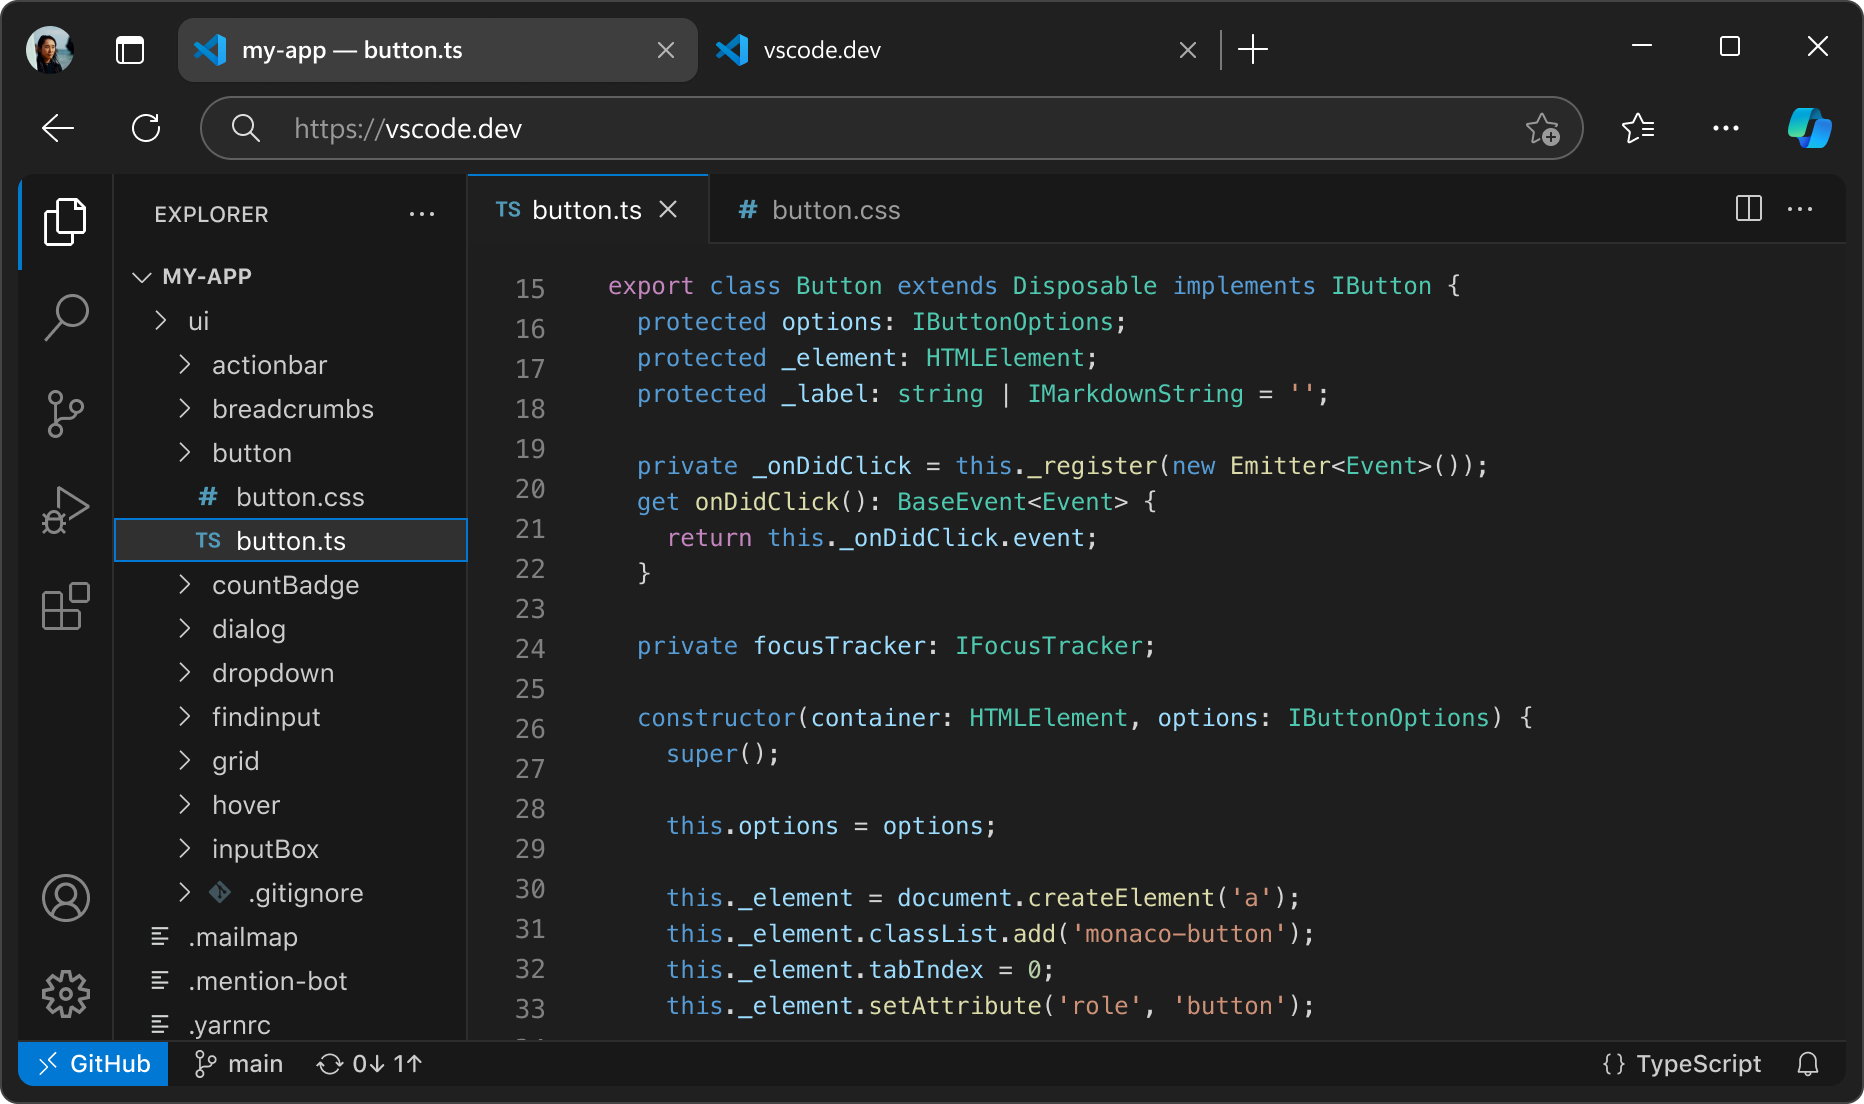
\includegraphics[width=0.85\textwidth]{figuras/docx/vscode-interfaz.png}
    \caption{Interfaz de Visual Studio Code}
    \label{fig:vscode}
\end{figure}

% =====================================================================
\section{Frameworks para desarrollo Mobile}
\label{sec:frameworks}

El desarrollo de aplicaciones móviles ha evolucionado en gran manera gracias a
la aparición de frameworks que permiten crear interfaces eficientes,
multiplataforma y optimizadas para dispositivos con recursos limitados. Estos
frameworks ofrecen herramientas, bibliotecas y entornos de trabajo que
simplifican el proceso de creación de aplicaciones al abstraer componentes
nativos y proporcionar estructuras reutilizables.

Entre los frameworks más utilizados se encuentran React Native, Flutter, Ionic,
Xamarin y Jetpack Compose.

{\small
\begin{longtable}{L{2.2cm} L{5.7cm} L{3.8cm} L{2.7cm}}
\caption{Comparación de frameworks de desarrollo Mobile}
\label{tab:frameworks}\\
\toprule
\textbf{Framework} & \textbf{Descripción} & \textbf{Características} &
\textbf{Ventajas} \\
\midrule
\endfirsthead
\toprule
\textbf{Framework} & \textbf{Descripción} & \textbf{Características} &
\textbf{Ventajas} \\
\midrule
\endhead
\bottomrule
\endfoot
React Native & Es un framework de Meta para construir aplicaciones nativas
para iOS y Android, usando JavaScript. Este framework usa el paradigma
fundamental de construcción de bloques de UI (componentes visuales con los que
interacciona el usuario) (Deloitte, 2019). &
\begin{tablista}
  \item Multiplataforma.
  \item Fast Refresh y Hot Reload.
  \item Acceso a componentes y APIs nativas.
  \item Gran comunidad y ecosistema amplio.
  \item Integración con librerías como Redux, Axios, Firebase.
\end{tablista} &
Alto rendimiento. Reutilización de código. Amplia compatibilidad. \\
\midrule
Flutter & Es un framework de código abierto de Google basado en Dart con motor
de render propio (Flutter, s.f.). &
\begin{tablista}
  \item Widgets personalizables.
  \item Animaciones.
  \item Hot Reload.
\end{tablista} &
UI consistente. Excelente rendimiento gráfico. \\
\midrule
Ionic & Ionic es un framework híbrido basado en tecnologías web (HTML, CSS,
JavaScript) que funciona mediante WebView. Permite construir aplicaciones con
enfoques multiplataforma usando Angular, React o Vue. Es especialmente útil
para aplicaciones orientadas a contenidos web o prototipado rápido (Ionic
Documentation, 2023). &
\begin{tablista}
  \item Multi-framework.
  \item Amplia colección de componentes UI.
  \item Soporte para Progressive Web Apps.
\end{tablista} &
Desarrollo rápido. Curva de aprendizaje baja. \\
\midrule
Xamarin & Xamarin es un framework de Microsoft basado en C\# y .NET, que
compila aplicaciones nativas para Android, iOS y Windows. Permite compartir
hasta 90\,\% de la lógica de negocio entre plataformas y se integra
profundamente con Visual Studio. Es utilizado ampliamente en entornos
empresariales (Microsoft, 2022). &
\begin{tablista}
  \item Acceso directo a APIs nativas.
  \item Integración con Visual Studio.
  \item Integración con .NET MAUI.
\end{tablista} &
Sólido para apps empresariales. Reutilización de lógica. \\
\midrule
Jetpack Compose & Jetpack Compose es el framework declarativo moderno de
Android, basado en Kotlin. Permite construir interfaces de usuario mediante
funciones composables, eliminando XML y ofreciendo mayor control del sistema y
rendimiento nativo. Es el estándar actual para desarrollar aplicaciones Android
modernas (Android Developers, 2024). &
\begin{tablista}
  \item UI declarativa.
  \item Integración con Android Jetpack.
  \item Animaciones avanzadas.
\end{tablista} &
Rendimiento máximo. Control total del sistema. \\
\end{longtable}
}
\fuente{Elaboración propia basada en (Deloitte, 2019); (Flutter, s.f.);
(Android Developers, 2024); (Microsoft, 2022).}

\conclusion{En conclusión, React Native destaca frente a los demás frameworks
debido a su equilibrio entre rendimiento y desarrollo multiplataforma, su
capacidad de generar componentes nativos le da mayor fluidez a diferencia de
Ionic y Flutter. Así también, permite desarrollar aplicaciones de forma
eficiente y se adapta al entorno de Android.}

\subsection{React Native}

React Native es un framework para la creación de aplicaciones nativas para iOS
y Android, creado por Meta (Facebook). Permite construir aplicaciones
multiplataforma utilizando JavaScript y React. A diferencia de las soluciones
híbridas tradicionales, React Native genera interfaces nativas, lo que permite
lograr un rendimiento cercano al desarrollo completamente nativo (React Native,
2025).

React Native se caracteriza por (Viera, s.f.):

\begin{itemize}
    \item \textbf{Componentes nativos:} Usa componentes de interfaz de usuario
    nativo en lugar de componentes web.
    \item \textbf{Hot reloading:} Permite ver cambios en tiempo real sin
    recompilar toda la app, acelerando el desarrollo.
    \item \textbf{Acceso a APIs nativas:} Permite integrar funcionalidades como
    cámara, GPS y notificaciones directamente del dispositivo.
    \item \textbf{Desarrollo Multiplataforma:} Escribe una sola vez y ejecuta en
    ambas plataformas (iOS y Android).
    \item \textbf{Gran Comunidad:} Amplia comunidad de desarrolladores y recursos
    disponibles.
    \item \textbf{Rendimiento:} Ofrece un rendimiento cercano al nativo gracias a
    su arquitectura.
    \item \textbf{Interfaz de Usuario:} Permite crear interfaces de usuario ricas
    y fluidas.
    \item \textbf{Integración con Librerías:} Compatible con librerías de
    terceros y APIs nativas.
    \item \textbf{Soporte para TypeScript:} Permite usar TypeScript para un
    desarrollo más robusto y seguro.
\end{itemize}

% =====================================================================
\section{Bases de datos de aplicaciones Móviles}
\label{sec:bases-datos}

Las bases de datos desempeñan un papel fundamental en el desarrollo de
aplicaciones móviles, ya que permiten almacenar, administrar y sincronizar la
información que utiliza el sistema durante su funcionamiento.

En el entorno móvil actual existen múltiples opciones tecnológicas, entre las
cuales destacan Firebase Firestore, SQLite, MongoDB Atlas, MySQL y PostgreSQL.

{\small
\begin{longtable}{L{2.1cm} L{5.6cm} L{3.5cm} L{3.2cm}}
\caption{Comparación de bases de datos para aplicaciones móviles}
\label{tab:bases-datos}\\
\toprule
\textbf{Base de Datos} & \textbf{Descripción} & \textbf{Características} &
\textbf{Ventajas} \\
\midrule
\endfirsthead
\toprule
\textbf{Base de Datos} & \textbf{Descripción} & \textbf{Características} &
\textbf{Ventajas} \\
\midrule
\endhead
\bottomrule
\endfoot
Firebase Firestore & Es una base de datos NoSQL en la nube que permite
sincronización en tiempo real y almacenamiento distribuido (Isaac, 2025). Su
base de datos principal, Cloud Firestore, es una solución NoSQL escalable
diseñada para sincronización en tiempo real, rendimiento móvil y arquitectura
serverless. &
\begin{tablista}
  \item Escalable.
  \item Documentos y colecciones.
  \item Soporte offline.
\end{tablista} &
\begin{tablista}
  \item Fácil integración móvil.
  \item Sin servidor.
  \item Arquitectura serverless.
  \item Integración con el ecosistema de Google.
\end{tablista} \\
\midrule
SQLite & Es una biblioteca en lenguaje C, es el motor de base de datos más
utilizado en el mundo. Se encuentra integrado en todos los teléfonos móviles y
en la mayoría de las computadoras, es de código abierto (SQLite Consortium,
2024). &
\begin{tablista}
  \item Escalable.
  \item Documentos y colecciones.
  \item Soporte offline.
\end{tablista} &
\begin{tablista}
  \item Fácil integración móvil.
  \item Ligera y de bajo consumo.
  \item Amplio soporte y estabilidad.
  \item Sin servidor.
  \item Tiempo real.
\end{tablista} \\
\midrule
MongoDB Atlas & Es un servicio de base de datos multicloud, simplifica la
implementación y gestión de bases de datos. Permite manejar grandes volúmenes
de datos, consultas avanzadas y procesamiento en la nube con altos niveles de
seguridad y escalabilidad (MongoDB, 2024) (Huang, 2020). &
\begin{tablista}
  \item Ligero.
  \item Transaccional.
  \item Estructura relacional.
\end{tablista} &
\begin{tablista}
  \item Ideal para uso offline.
  \item Ampliamente soportado.
  \item Integración nativa con la nube.
  \item Funciones avanzadas de seguridad.
\end{tablista} \\
\midrule
MySQL & MySQL es un sistema de gestión de bases de datos relacional (RDBMS) de
código abierto ampliamente utilizado en aplicaciones web y móviles.
Originalmente desarrollado por MySQL AB y actualmente mantenido por Oracle
Corporation, MySQL se ha consolidado como una solución flexible, rápida y
confiable para gestionar datos estructurados (DuBois, 2013); (Corporation,
2024). &
\begin{tablista}
  \item Lenguaje SQL para definición y manipulación de datos.
  \item Soporte para múltiples motores de almacenamiento.
  \item Ejecución de transacciones ACID.
  \item Alta compatibilidad con lenguajes de programación.
\end{tablista} &
\begin{tablista}
  \item Flexible.
  \item Escalable.
  \item Adecuada para grandes volúmenes.
\end{tablista} \\
\midrule
PostgreSQL & Sistema de gestión de bases relacional ampliamente utilizado.
Destaca por su arquitectura orientada a objetos, su capacidad para manejar
grandes volúmenes de datos y su soporte para consultas complejas, extensiones y
tipos de datos personalizados. &
\begin{tablista}
  \item SQL.
  \item Robusto.
  \item Seguro.
  \item Gestión avanzada de concurrencia.
  \item Soporte para JSON y JSONB para datos semiestructurados.
\end{tablista} &
\begin{tablista}
  \item Ideal para Backend estructurado.
  \item Rendimiento estable.
  \item Perfecto para aplicaciones móviles.
\end{tablista} \\
\end{longtable}
}
\fuente{Elaboración basada en (Corporation, 2024); (Huang, 2020); (MongoDB,
2024).}

\conclusion{En conclusión, Firebase Firestore es la mejor alternativa, por su
arquitectura NoSQL, reduce la complejidad del Backend y es escalable.}

\subsection{Firebase}

Firebase es una plataforma en la nube desarrollada por Google, facilita el
desarrollo de aplicaciones, bases de datos en tiempo real, autenticación y
hosting. Esta herramienta permite enviar notificaciones push y analizar el
rendimiento de las apps (Isaac, 2025).

En la actualidad, Firebase integra servicios modernos como Cloud Firestore,
Google Analytics 4, App Check, Data Connect y Firebase Studio, lo que la
convierte en una solución completa para proyectos actuales que buscan
escalabilidad, seguridad y analítica avanzada (López Mora, 2025).

% =====================================================================
\section{Modelos de Lenguaje Extenso (LLM)}
\label{sec:llm}

{\small
\begin{longtable}{L{2.2cm} L{4.4cm} L{4.0cm} L{3.8cm}}
\caption{Comparación de modelos de lenguaje extenso}
\label{tab:llm}\\
\toprule
\textbf{Modelo} & \textbf{Descripción} & \textbf{Características} &
\textbf{Ventajas} \\
\midrule
\endfirsthead
\toprule
\textbf{Modelo} & \textbf{Descripción} & \textbf{Características} &
\textbf{Ventajas} \\
\midrule
\endhead
\bottomrule
\endfoot
OpenAI GPT-4 & Modelo avanzado de OpenAI con capacidades de razonamiento y
comprensión contextual profunda. & Alta precisión; multimodal; entrenado con
gran cantidad de parámetros. & Respuestas coherentes; excelente para tareas
complejas. \\
\midrule
Gemini (Google) & Modelo multimodal de Google capaz de procesar texto, imágenes
y audio. & Optimización contextual; integración nativa con Google. & Muy
rápido; fuerte rendimiento en análisis multimodal. \\
\midrule
Claude 3 & Modelo de Anthropic centrado en seguridad y precisión. &
Entrenamiento ético; respuestas estables y seguras. & Ideal para tareas largas
y análisis profundo. \\
\midrule
Llama 3 & Modelo open-source de Meta, altamente eficiente y adaptable. & Open
source; optimización local; adaptable. & Perfecto para personalización y
despliegue en servidores propios. \\
\end{longtable}
}
% TODO: en el documento Word esta tabla no tenía fila de "Fuente".
\fuente{\pendiente{indicar la fuente de la tabla.}}

\subsection{OpenAI}

OpenAI ofrece modelos de lenguaje avanzados, como GPT-4, que permiten realizar
tareas complejas de procesamiento de lenguaje natural, generación de texto,
análisis semántico, recomendaciones personalizadas y soporte conversacional.
Estos modelos se integran mediante API y pueden ser empleados dentro de
aplicaciones móviles para funciones inteligentes.

Los modelos de OpenAI están basados en la arquitectura Transformer, que permite
procesar grandes volúmenes de información con alta precisión. Además, OpenAI
proporciona herramientas que facilitan la integración de estos modelos en
distintos entornos tecnológicos, incluyendo plataformas web, sistemas de
atención al cliente, análisis de datos y automatización de procesos
empresariales. Los modelos aprenden a partir de enormes conjuntos de datos, lo
que les permite comprender contextos complejos, mantener conversaciones
coherentes y generar contenido creativo en múltiples idiomas. Por otra parte,
OpenAI trabaja en la mejora continua de la seguridad y la ética en el uso de
IA, implementando mecanismos para minimizar sesgos, evitar desinformación y
garantizar que los resultados sean confiables y útiles para los usuarios
finales.

% =====================================================================
\section{Herramientas}
\label{sec:herramientas}

\subsection{Control de versiones}

El control de versiones es un sistema que ayuda a rastrear y gestionar los
cambios realizados en un archivo o conjunto de archivos, principalmente
utilizado por ingenieros de software para hacer seguimiento a las
modificaciones realizadas en el código fuente (B, 2025).

Para esto utilizaremos:

\begin{enumerate}
    \item \textbf{Git:} Es un sistema de control de versiones distribuido,
    gratuito y de código abierto diseñado para manejar proyectos pequeños, como
    también proyectos muy grandes de forma rápida y eficiente (Git, s.f.).
    \item \textbf{GitHub:} Es un servicio basado en la nube que aloja un sistema
    de control de versiones (VCS) llamado Git. Éste permite a los
    desarrolladores colaborar y realizar cambios en proyectos compartidos, a la
    vez que mantienen un seguimiento detallado de su progreso (B, 2025).
\end{enumerate}

\subsection{Herramientas de Gestión}

Las herramientas de gestión de proyectos están especialmente diseñadas para
asistir a un empleado o equipo en la gestión eficaz de sus proyectos y tareas
(Gurnov \& Wrike (W.), 2025). Estas herramientas son utilizadas para la
organización, planificación, seguimiento y aseguramiento de calidad del
proyecto.

\begin{itemize}
    \item \textbf{Trello:} Es una herramienta flexible para la gestión del
    trabajo, basado en tableros Kanban que facilita la organización visual de
    tareas mediante listas y tarjetas (Atlassian, 2023). Su enfoque intuitivo
    permite coordinar actividades, asignar responsabilidades y monitorear el
    avance de cada fase del proyecto.
\end{itemize}
